%\documentclass{tise_style}
%\usepackage{natbib}
%Having trouble getting tise_style to compile correctly in RStudio, will re-run it with this before submission

%-----------------------------------------------------------------------------------------------------
%Substitute this all with tise_style
\documentclass[12pt]{article}
\usepackage{natbib}  % used for citations
\usepackage[parfill]{parskip} %used for formatting style of text
\usepackage{url}
\usepackage{graphicx}
\usepackage{setspace}
\usepackage{fancyvrb}
% Sets margins to 1 in
%\addtolength{\oddsidemargin}{-.5in}%
%\addtolength{\evensidemargin}{-.5in}%
%\addtolength{\textwidth}{1in}%
%\addtolength{\textheight}{1.3in}%
%\addtolength{\topmargin}{-.8in}%
%-----------------------------------------------------------------------------------------------------



\title{Enter our title here}

\author{Tessa Mcdonnel, Shannon Pileggi,  \\Statistics Department, California Polytechnic State University, San Luis Obispo}
%\author{Shannon Pileggi \\Statistics Department, California Polytechnic State University, San Luis Obispo}




\begin{document}


\maketitle

\section{Introduction}

\doublespacing

Questions: 

How do I say that LaTeX is compatible with datacamp?

I can't find the swirl package on mendeley so im not sure how to add that.

How did the linking with LMS process go?


It is no suprise that technology plays a vital role in practicing statistics and as the technological revolution continues to
unfold, the use of statistical software has become increasingly emphasized in education \citep{AmericanStatisticalAssociation2016}. By integrating the
capabilities of technology in statistics courses, students can explore fundamental concepts by analyzing and
interpreting real data sets \citep{Chance2007, Hardin2015, Horton2014}, giving them an authentic view of how statistics is practiced outside of the
classroom \citep{Wang2017}. The revised 2016 \textit{Guidelines for Assessment and Instruction in Statistics Education}
(GAISE) College Report has also prompted the use of more technology in introductory statistics courses, encouraging educators
to use technology "as a way to explore conceptual ideas and enhance student learning" \citep{AmericanStatisticalAssociation2016}.

The goal for any statistics course is to help students develop the ability to think statistically
\citep{AmericanStatisticalAssociation2016}.
Introducing technology into the curriculum can greatly strengthen this ability by illustrating statistical concepts such as
variability, randomness and hypothesis testing. Although numerous statistical technologies exist, R and R Studio
provide extensive statistical capabilites (free of charge) and are commonly used in statistics courses \citep{Chance2007}. R
allows students to explore real-world data sets which can not only enhance their understanding of concepts, but can also spark
an interest in the domain of statistics \citep{Wang2017}.

With this increased use of R in classrooms, there is a need for an effective way to get students familiar with statistical software
\citep{Baumer2014}. While R software provides users with extraordinary capabilities, there is no doubt a steep learning curve. To facilitate
this transition to R programming, popular interactive teaching technologies have been created including swirl (** need to cite package**), LearnR and TryR. 
These tools allow students to work through coding problems while recieving immediate feedback in and out of the classroom. swirl is an
open source R package that allows students to learn R programing in their R console. This interactive learning tool
contains several pre-existing lessons but what makes swirl so popular is its versitality; educators can also create their own
lesson to fit the curriculum and assign it to students \citep{Carchedi2014}.
While swirl can be linked to a Massive Open Online Courses (MOOCs) like Coursera through API, integration of learning management 
systems (LMS) is not available for the classroom. 

\textbf{Learn R section}


*Try R website  \url{http://tryr.codeschool.com} i dont know how to cite this with mendeley*

TryR (Code School 2014) is a web-based program but is not open source. Since public content authoring
is not available, educators are limited on what they can teach their students. The R console can be intimidating to
new statistics students so an advantage of a web-based teaching tool is
the clean and easy to use interface. This is an important quality given that a lot of the time students struggle more with
software than the statistical concepts themselves \citep{Hare2017}. When students only need their web browser to participate,
all installation complications are avoided and valuable class time can be focused on the statistics, not computer issues.

The purpose of this article is to introduce a relatively new technology, DataCamp, which incorporates the best
qualities from the teaching tools mentioned above.

DataCamp has the same reproducable capabilities as swirl but is a web-based application; educators can
create their own courses that coincide with their lessons and students can access the course without installing R.
Courses are available through the DataCamp website and students can access the lesson through their web-browser on a laptop,
tablet or moble device, making the courses accessible to anyone with an internet connection. 
The DataCamp website offers pre-existing free community courses as well as specialized \textit{Premium} classes that you need to purchase. 
However, when used for academic purposes the \textit{Premium} DataCamp content is also free for up to six months.
Any college educator can create a classroom group on the DataCamp website, add student's to the group, assign 
\textit{community} courses, \textit{Premium} courses, and even a course that they've developed themselves. 
The collection of \textit{community} courses available on DataCamp inlcude a wide range of topics from \textit{Introduction to R} to
\textit{Quantitative Risk Management in R} so novice through advanced programming students benefit.

DataCamp can be used in the classroom in a number of ways: as traditional homework assignments, as an
activity during lab periods, as pre-class assignments for a flipped classroom, and even as a test or assessment tool.

A feature that sets DataCamp apart from competing technologies is the ability to track student progress. Educators
can set deadlines for assignments and easily see not only when students complete an assignment but also which sections the
students had trouble with in a detailed report (need to cite teach page of website). Student scores can be automatically updated to a
current gradebook when you link the schools' learning management system (LMS) to DataCamp, allowing for a smooth integration of student work.

Each chapter in a DataCamp course is made up of modular exercises. Modularity is critical component in designing a statistical
learning tool because it allows independent pieces to be easily added, modified or removed from the entire functionality
\citep{Hare2017}. Course exercises can be added, modified, or deleted as new topics arise and instructors can tailor
these exercises to meet the needs of a particular class. The only disadvantage of the modularity feature is that the sessions
are not cummulative; every exercise begins with a clear workspace so an object defined in a previous exercise needs to be
defined again.

Each of these exercises can be given a number of redeemable points which the students can see when they begin
the exercise, introducing a gamification feature to the learning experience. Students can view the exercise `hint' option and 30 percent
of the available points are deducted; all points are deducted if they ask for the solution.  If the student completes the exercise without
any help they will recieve the full points. When in a classroom group, students can view their
progress (points and chapters completed) as well as then progress of their peers. This can help students perform better
because they want to be on par with the rest of the class; furthermore, when students can see the number of available points
for an exercise it can motivate them to meet their personal achievement goals. \citep{Chang2016}.


\section{How to Use DataCamp}

\subsection{Pre-existing R courses}
In order to utilize 
DataCamp's \textit{classroom} benefits, first create an academic group on the website \url{https://www.datacamp.com/groups/education}.
After your university information has been verified and the classroom account has been approved, you can facilitate student access
by either creating a group through the DataCamp website or linking directly to your LMS.


(idk if this helps to say or is obvious) Add students by their university email address on the \textit{Members} tab and link the account to your LMS.)



\subsection{Creating a DataCamp Course}
To build a course on DataCamp you will first need to create a DataCamp account by visiting \url{www.datacamp.com/teach} and
a GitHub account \url{https://github.com}. The simplest way to begin building the course is to use the template course files from the 
\texttt{Create DataCamp Course} dialog. This will automatically create a GitHub repository that is linked to DataCamp; any changes that are
make through DataCamp will update the GitHub repository and vice versa. Every DataCamp course is linked through GitHub version control,
allowing statistics educators to easily collaborate and reproduce code. To add collaborators to the course, go to the course repository
on GitHub and under \texttt{Settings} you can enter the user names of collaborators. Collaborators who are not the primary author need 
to uncheck `My Courses' in order to view and contribute to the repository.



The newly created GitHub repositories will contain three files: 

1) \texttt{README.md}

2) \texttt{course.yml}

3) \texttt{chapter1.Rmd}


\texttt{Readme.md} contains helpful information of how to get started, citing resourses to learn more about the process.
\texttt{course.yml} is a file that contains general information about the course you're creating: title, university, description,
difficulty level, ect.
\texttt{chapter1.Rmd} is a template chapter file with examples of 'normal' interative coding exercises and multiple choice questions.
To add more chapters to an R course, create new files in the repository and name them \texttt{chapter1.Rmd}, \texttt{chapter2.Rmd},
\texttt{chapter3.Rmd}, ect.

When starting to create a DataCamp course, it is helpful to view code from pre-existing community courses which can be found on GitHub.
You can use these files as a guide to build your own course or duplicate the repository and tailor the content to fit specific needs.
The DataCamp github repository contains links to the code for several available courses; one of the most helpful when starting to build a course 
is \url{https://github.com/datacamp/courses-intro-to-r} which contains the source files for the `Intoduction to R' course.

Educators are able to edit their courses in a number of ways but the 'Teach Editor' located in the teach dashboard is the
most straight forward editor. The 'Teach Editor' is specifically designed to make the creation process of a DataCamp course
as painless as possible, allowing writers to edit, preview, save changes and synchronize to a GitHub repository. Editing can
also be done through GitHub's online editor and through git locally but these methods do not allow for automatic content
viewing.

DataCamp courses may contain 3 different types of exercises: Normal, Multiple choice, and video.

A \texttt{NormalExercise} is an exercise that prompts a user to submit code. The components of this include: lesson section, instructions, pre-exercise code, sample code, hint, solution and a submission correctness testing coded (SCT). However, the interface for students (or the 'Preview
mode) only includes the lesson, Instructions, R script panel and a R console panel (Figure~\ref{fig:code1}).


\begin{figure}
\caption{This code does this}
\begin{verbatim}[frame=single]
--- type:NormalExercise lang:r xp:100 skills:1 key:9a4fea2da
## Visualizing quantitative data in R

We can visualize quantitative data with a *histogram*.

To create a histogram in R, use the syntax:
`hist(dataset$quant_var)`

*** =instructions
- Create a histogram of the `wage` variable from the 
`CPS85` data set.
*** =hint
Follow the format from the lesson: `hist(dataset$variable)`
with specified data set and variable.
*** =pre_exercise_code
```{r}
library(mosaicData)
```
*** =sample_code
```{r}
# Create histogram of the wage variable
```
*** =solution
```{r}
# Create histogram of the wage variable 
hist(CPS85$wage)
```
*** =sct
```{r}
test_function("hist", args = "x", incorrect_msg = 
"Make sure you specify the `CPS85` data set
and `wage` variable.")
```

\end{verbatim}
\label{fig:code1}
\end{figure}

\begin{figure}[h]
  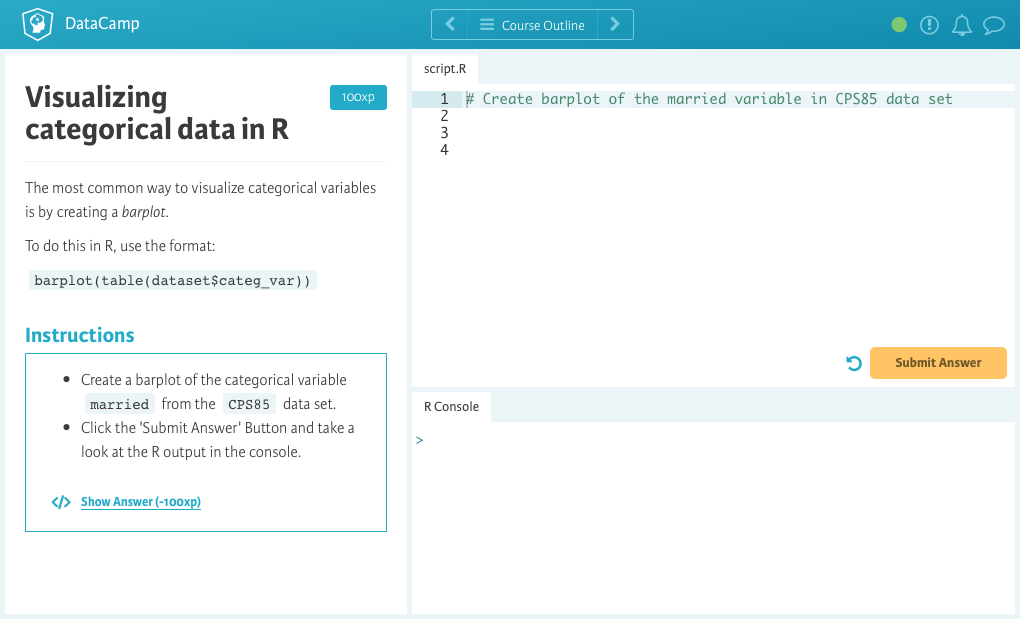
\includegraphics[scale = 0.19] {preview.jpg}
\end{figure}


Whenever a new exercise is added, DataCamp automatically produces the top line in the editor. The header specifies the type
of exercise \texttt{type}, language \texttt{lang}, available points \texttt{xp}, skills learned \texttt{skills} and a \texttt{key}. The key acts as a unique
identifier for that exercise, allowing you to modify the content without losing any student data. Currently, DataCamp offers
eight different skills which are defined by numbers 1-8. The skills and their corresponding numbers can be found in the DataCamp
documentation \url{https://www.datacamp.com/teach/documentation#tab_gamification}. 
In the above exercise code, the \texttt{type} is Normal, the language is R, the available points is 100 and the skills learned is 1 (which 
corresponds to R Programming). DataCamp assigns 100 points to normal coding exercises but this value can be modified depending on
difficulty level. After students have completed the exercise, they can check their personal profile to see how many points they earned.


In the `Assignment' portion of the exercise, instructors can add additional information about the assignment that will help
students understand and complete the instructions. The `Instructions' section contains the actual task the student is
asked to execute; instructors can also include a `Hint' for extra guidence (optional). The 'pre-exercise code' sets up the workspace for 
the student; this section will contain code to import data sets, install packages and any other operation that you want to be available to
students. The 'sample code' section contains code or notes that students view in the R script panel. Students also use the R script panel to write
the code that solves the tasks in the instructions. The correct answer to an exercise is coded in the 'solution' section
and when the student clicks the `Submit Code' button, their answer passes through the SCT code where their code is checked for errors.


The submission correctness testing code (or SCT) automatically assesses if the correct code was submitted. If a student submits an 
incorrect answer, they will receive immediate feedback on what they are doing wrong and the system will guide them to the right answer.
Instructors can use the default feedback that DataCamp automatically generates or write their own custom messages. For example, figure blank
contains the default feedback for an incorrect submission of the \texttt{hist()} function.




\begin{figure}
\caption{This code does this}
\begin{Verbatim}[frame=single]

Student types:
histogram(dataset$var_name)

Default message:
Have you called hist()?

Student types:
hist(var_name)

Default message:
Check your call of hist(). Did you correctly specify 
the argument x? Evaluating the expression you specified
caused an error.

Student types:
hist(dataset$misspelled_var)

Default message:
Check your call of hist(). Did you correctly specify the
argument x? 
It is a NULL, while it should be a numeric vector.


\end{Verbatim}
\label{fig:code1}
\end{figure}


















The default feedback is meaningful and specific; most of the time custom 
messages are not necessary unless there is a common problem that student are struggling with in which more unique feedback is necessary. 
DataCamp provides a helpful R package called 'testwhat' which acts as a guide to writing and using SCTs (this can be accessed on DataCamp's GitHub 
repository: \url{https://github.com/datacamp/testwhat/wiki}. 
'testwhat' contains functions that can test different types of problems including loops, object definitions, printed output, functions, ect.
The submission correctness testing code compares the ideal answer (from the solution) to the students answer. Different
arguements can be added to the test functions to alter the testing process and automatic feedback. (**do I cite datacamp website here?**)

%add an example of a test_function sct.... maybe plot




The \texttt{MultipleChoiceExercise}, as you would expect, contains a question and a list of various answers. Instructors write the questions in the 'lesson'
portion of the exercise and offer solutions in the 'Insructions' section. Similar to the 'normal' coding exercises, the lesson, instructions, pre-exercise 
code and SCTs have to be specified but sample and solution code do not. DataCamp offers two types of multiple choice questions: simple and regular. 
The simple multiple choice exercises are used for questions that do not require the R console or any R output. Regular multiple choice exercises 
allow instructors to pre-program objects or plots that the student needs to access to answer the question. Both types of multiple choice exercises 
are straight forward to write can act as quick checks for understanding throughout the chapter.

\begin{figure}
\caption{This code does this}
\begin{Verbatim}[frame=single]
--- type:PlainMultipleChoiceExercise lang:r xp:50 skills:1 key:9707072219
## Quick check 2

What can R be used for?

*** =instructions
- Graphing data
- Analyzing data
- Calculations
- All of the above

*** =hint
R software can be used for all of these things.

*** =pre_exercise_code
```{r}

```

*** =sct
```{r}

msg_bad <- "That is not correct"
msg_success <- "Exactly! R can do all of these things."
test_mc(correct = 4, feedback_msgs = c(msg_bad, msg_bad, msg_bad, msg_success))
```
\end{Verbatim}
\end{figure}

%add example of regular multiple choice exercise --> use Quick check 2 from lab 8

Video exercises act as in instructional video addition to a DataCamp course; instructors can add short videos of them explaining concepts and with 
relevent slides that appear in the background. The DataCamp website \url{https://www.datacamp.com/teach/documentation#tab_code_exercises} provides 
more detail on the content of the various exercises. 


Tips for smoother course development process:
    + Using LaTeX math symbols to display greek letters, operators, ect.
    + When using datacamp and github, press 'refresh' when available on the screen

All DataCamp courses will have a course badge and most will use data sets and R packages. Information on how to add data sets and images
can be found in DataCamps 'Teach' documentation \url{https://www.datacamp.com/teach/documentation} under the 'Upload Assets' tab. However,
there is currently no information on DataCamp about integrating R packages. To use R packages in a course, you will need to create a new file
in the GitHub course repository named \texttt{requirements.r}. The file should contain: \texttt{devtools::install\_version}, package name and version for 
every package you use in the DataCamp course. For example, following code will add the \texttt{ggplot2} and \texttt{mosaic} packages to the repository.

\begin{verbatim}
devtools::install_version("ggplot2", "2.2.0")
devtools::install_version("mosaic", "0.14.4")
\end{verbatim}
In order for DataCamp to recognize this new file, you will need to add \texttt{from: r-base-prod:27} to the \texttt{course.yml} file.

LaTeX is compatable with DataCamp course builders can use LaTeX math symbols to display Greek letters, formulas, ect. For example:
\begin{verbatim}
$H_0$: $p = 0.07$
$H_a$: $p \neq 0.07$
\end{verbatim}

translates to:

$H_0$: $p = 0.07$

$H_a$: $p \neq 0.07$


%Check this out, Schubert said this \cite{Schubert13}.


%Check this out, Campbell said this \cite{Campbell02} regularly, but cite this in parentheses \citep{Campbell02}.


%Check this out, Chi said this \cite{Chi81}.

%Use this for final submission
%\bibliographystyle{ECA_jasa}
\bibliographystyle{plainnat}
\bibliography{library}




\end{document}
